%% MANUALE DELL'APPLICAZIONE
\section{Introduzione}
\subsection{Cos'è Monolith SDK?}
Monolith SDK è un pacchetto \glossario{Meteor} che consente la creazione di bolle interattive in ambiente \glossario{Rocket.chat}.\\
Lo Sviluppatore avrà la possibilità di usare i componenti della SDK per costruire le proprie bolle da integrare a quelle già esistenti sulla piattaforma di \glossario{Rocket.chat}.
\subsection{Scopo del documento}
Questo documento rappresenta il manuale utente per l'applicazione Monolith SDK nel quale vengono descritte dettagliatamente tutte le caratteristiche dell'applicativo utilizzabili dall'utente.
Il manuale sarà diviso in sezioni per essere maggiormente comprensibile e spiegherà le varie componenti che l'utente potrà utilizzare per costruire la propria bolla.
\subsection{Glossario}
In modo tale da evitare ambiguità di linguaggio e massimizzare la comprensione, i termini tecnici, di dominio, gli acronimi e le parole che necessitano di essere chiarite, sono riportate nel documento \gloss .\\
Ogni occorrenza di vocaboli presenti nel Glossario è marcata da una \glossario{} maiuscola in pedice.

\section{Utilizzo}

\subsection{Layout}
\subsubsection{VerticalLayout}
Layout verticale che conterrà i componenti della bolla e li posizionerà ognuno sotto al proprio precedente. La props \textit{hide} permette di nascondere la vista del layout (tramite valori \textit{true/false}).
\begin{center}
\underline{\textit{Utilizzo}}
\begin{lstlisting}
<VerticalLayout hide={}>
<Children/>
<Children/>
.
.
.
</VerticalLayout>
\end{lstlisting}
\end{center}
\newpage

\subsubsection{HorizontalalLayout}
Layout orizzontale che conterrà i componenti della bolla e li posizionerà ognuno di fianco al proprio precedente. La props \textit{hide} permette di nascondere la vista del layout (tramite valori \textit{true/false}).
\begin{center}
\underline{\textit{Utilizzo}}
\begin{lstlisting}
<HorizontalLayout hide={}>
<Children/>
<Children/>
.
.
.
</HorizontalLayout>
\end{lstlisting}
\end{center}

\subsection{Components}
\subsubsection{CheckBoxList}
Una lista di Checkbox, i dati del CheckButton cliccato vengono ritornati tramite la funzione getCheck.
\begin{center}
\underline{\textit{Utilizzo}}
\begin{lstlisting}

<CheckBoxList
classes= // CSS classes
options={opt}
getCheck={this.fun}
/>
\end{lstlisting}
\underline{\textit{Esempio opzioni}}
\begin{lstlisting}
var opt=[{id: 1, value: 'Hello World'},{id: 2, value: 'value'}];
\end{lstlisting}
\underline{\textit{Funzione di ritorno}}
\begin{lstlisting}
function fun(m) {...}

m={id:'', value:'', check:''};
\end{lstlisting}
\end{center}

\subsubsection{CheckButton}

Componente Checkbox, i suoi dati vengono ritornati (ad ogni click) tramite la funzione getCheck.
\begin{center}
\underline{\textit{Utilizzo}}
\begin{lstlisting}
<CheckButton
id= ""
classes= // CSS classes
getCheck={this.fun}
value="" // Valore CheckButton
/>
\end{lstlisting}
\underline{\textit{Funzione di ritorno}}
\begin{lstlisting}
function fun(m) {...}

m={id:'', value:'', check:''};
\end{lstlisting}
\end{center}

\subsubsection{ComboBox}
Semplice elemento ComboBox. La funzione di ritorno riceve l'elemento selezionato.
\begin{center}
\underline{\textit{Utilizzo}}
\begin{lstlisting}
<ComboBox
id= ""
classes= // CSS classes
options={["a","b","c"]} //array of options
getSelection={this.fun}
/>
\end{lstlisting}
\end{center}

\subsubsection{Image}
Semplice elemento Immagine senza funzione di ritorno.
\begin{center}
\underline{\textit{Utilizzo}}
\begin{lstlisting}
<Image
id= ""
classes= // CSS classes
src= // like HTML "src" attribute
alt=  // like HTML "alt" attribute
width=  // like HTML "width" attribute
height=  // like HTML "height" attribute
/>
\end{lstlisting}
\end{center}

\subsubsection{ImageButton}
Elemento Immagine cliccabile come pulsante. La funzione di ritorno viene avviata quando l'immagine viene cliccata.
\begin{center}
\underline{\textit{Utilizzo}}
\begin{lstlisting}
<ImageButton
id= ""
src= // like HTML "src" attribute
alt=  // like HTML "alt" attribute
width=  // like HTML "width" attribute
height=  // like HTML "height" attribute
handleClick={this.fun}
/>
\end{lstlisting}
\end{center}
\newpage

\subsubsection{LineEdit}
Casella di testo editabile. La funzione "fun" salva il testo digitato e viene chiamata ad ogni modifica.
\begin{center}
\underline{\textit{Utilizzo}}
\begin{lstlisting}
<LineEdit
id= ""
classes= // CSS classes
updateState={this.fun}
value="default value"
/>
\end{lstlisting}
\end{center}

\subsubsection{LineEditComboBox}
Elemento formato da una casella di testo editabile e una ComboBox.\\
La funzione "fun1" riceve il testo dalla LineEdit mentre "fun2" l'opzione selezionata dal ComboBox.
\begin{center}
\underline{\textit{Utilizzo}}
\begin{lstlisting}
<LineEditComboBox
idle= // lineEdit id
idcb= // comboBox id
classesle= // lineEdit CSS classes
classescb= // comboBox CSS classes
textUpdate={this.fun1}
options={["a","b","c"]} //array of option
comboUpdate={this.fun2}
/>
\end{lstlisting}
\end{center}

\subsubsection{LineEditPushButton}
Elemento formato da una casella di testo editabile e un pulsante cliccabile.\\
La funzione "fun" riceve il testo dalla LineEdit quando il PushButton viene cliccato.
\begin{center}
\underline{\textit{Utilizzo}}
\begin{lstlisting}
<LineEditPushButton
idle= // lineEdit id
idpb= // pushButton id
classesle= // lineEdit CSS classes
classespb= // pushButton CSS classes
getText={this.fun}
buttonName="button name"
/>
\end{lstlisting}
\end{center}

\subsubsection{PushButton}
Pulsante cliccabile. La funzione "fun" viene eseguita al click sul pulsante.
\begin{center}
\underline{\textit{Utilizzo}}
\begin{lstlisting}
<PushButton
id= ""
classes= // CSS classes
handleClick={this.fun}
buttonName="button name"
/>
\end{lstlisting}
\end{center}

\subsubsection{RadioButtonGroup}
Elemento formato da un gruppo di RadioButton. La funzione "fun" restituisce l'opzione selezionata ad ogni cambiamento.
\begin{center}
\underline{\textit{Utilizzo}}
\begin{lstlisting}
<RadioButtonGroup
classes= // CSS classes
options={["a","b","c"]} //array of options
getValue={this.fun}
/>
\end{lstlisting}
\end{center}

\subsubsection{TextAreaButton}
Elemento area di testo editabile ed un PushButton.\\
La funzione "fun" riceve il testo dalla TextArea quando il PushButton viene cliccato.
\begin{center}
\underline{\textit{Utilizzo}}
\begin{lstlisting}
<TextAreaButton
idta= // textArea id
classesta= // textArea CSS classes
idpb= // PushButton id
classespb= // CSS classes
getText={this.fun}
width= // textarea width
height= // textarea height
buttonName= // button name
/>
\end{lstlisting}
\end{center}
\newpage
\subsubsection{TextAreaComboBox}
Elemento area di testo editabile ed un ComboBox.\\
La funzione "fun1" riceve il testo dalla TextArea mentre "fun2" l'opzione selezionata dal ComboBox.
\begin{center}
\underline{\textit{Utilizzo}}
\begin{lstlisting}
<TextAreaComboBox
idtx= //textArea id
classestx= // textArea CSS classes
idcb= //combobox id
classescb= // combobox CSS classes
width= // textarea width
height= // textarea height
textUpdate={this.fun1}
options={["a","b","c"]} // array of options
comboUpdate={this.fun2}
/>
\end{lstlisting}
\end{center}

\section{Bolle}
Vengono fornite alcune bolle tipo le quali vengono create tramite il menù presente nella SideArea1.\\

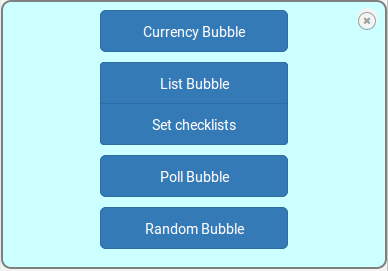
\includegraphics[scale=0.75]{img/menu.png}
\newpage
\subsection{CurrencyBubble}
La \textit{CurrencyBubble} è una bolla che funge da convertitore di valuta.
\\Una volta selezionata dal menù la si può configurare impostando la valuta di base, di uscita ed il valore da convertire.\\

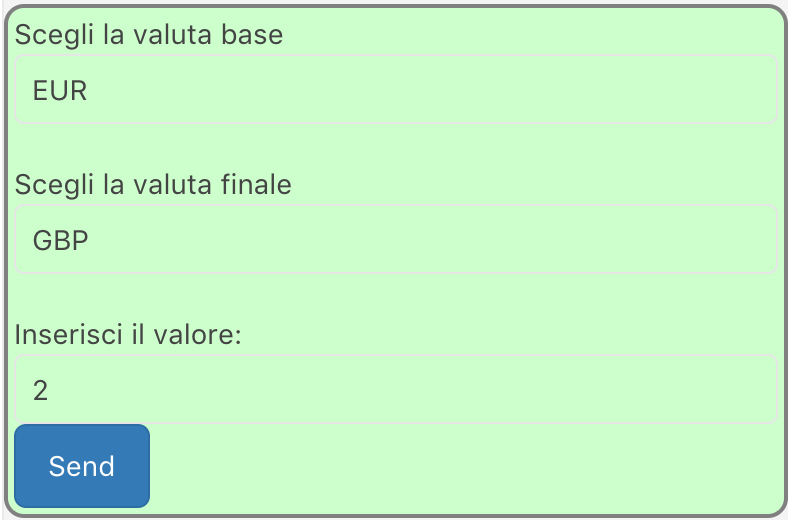
\includegraphics[scale=0.75]{img/currConfig.png}
\\
Una volta inviata cliccando su \textbf{Send} il risultato sarà:\\

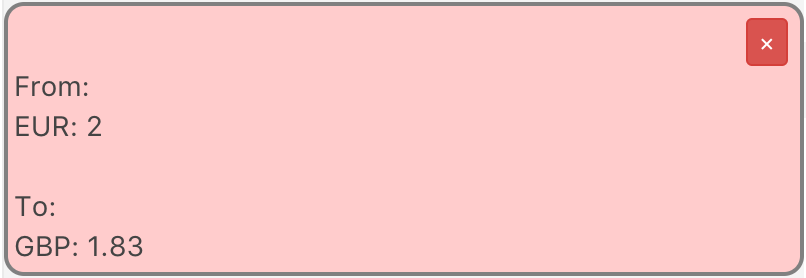
\includegraphics[scale=0.75]{img/curr.png}
\subsection{ListBubble}
La \textit{ListBubble} è una bolla che permette di creare una propria lista di elementi \textit{CheckButton}. \\
Può essere usata, ad esempio, per una classica lista della spesa o per una "ToDoList".

\subsection{PollBubble}
La \textit{PollBubble} è una bolla che permette di creare un sondaggio da lanciare ai membri della chat in questione.\\
Una volta arrivati al menù di configurazione si impostano la domanda e le varie opzioni (che si possono aggiungere con il pulsante \textbf{Add}).
\\

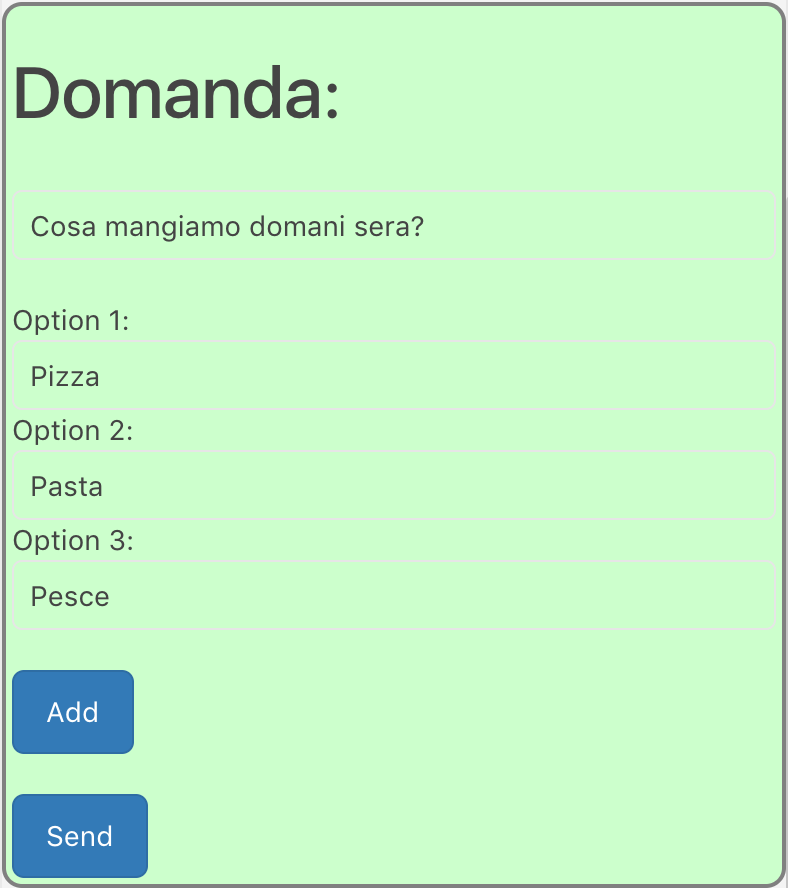
\includegraphics[scale=0.75]{img/pollConfig.png}
\\
Una volta inviata cliccando su \textbf{Send} il risultato sarà:\\

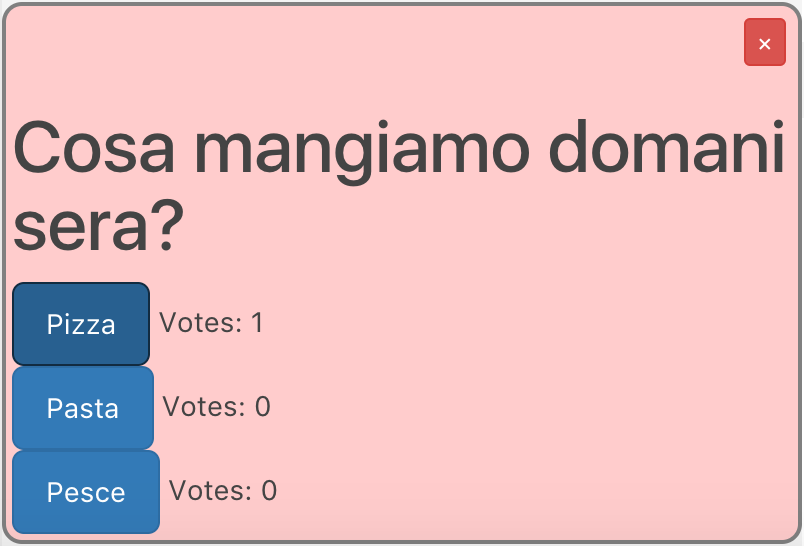
\includegraphics[scale=0.74]{img/poll.png}
\\
Ora che la bolla è stata creata sarà possibile votare cliccando sull'opzione desiderata.
\subsection{DiceBubble}
La \textit{DiceBubble} è una bolla che lancia un certo tipo di dado (a scelta in base al numero di facce) e ne ritorna un risultato casuale.\\
Dal menù di configurazione bisognerà scegliere il numero di facce del dado.\\

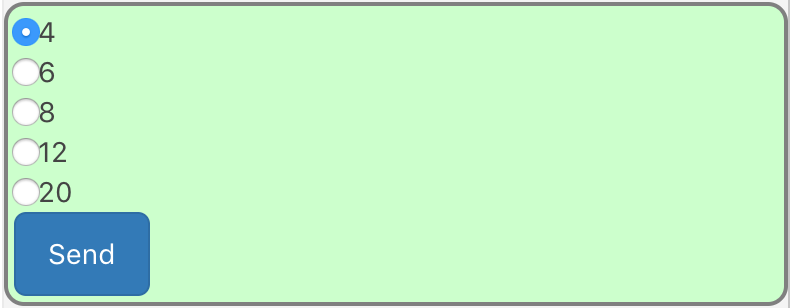
\includegraphics[scale=0.75]{img/randConfig.png}
\\
Una volta inviata cliccando su \textbf{Send} il risultato sarà:\\

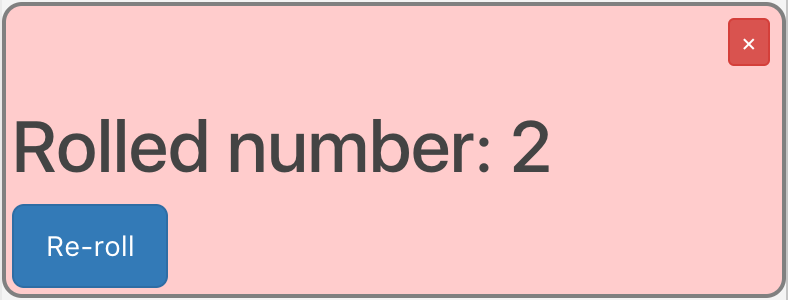
\includegraphics[scale=0.75]{img/rand.png}
\\
Attraverso il pulsante \textbf{Re-roll} si potrà rilanciare il dado.

\newpage

\section{DEMO - Lista con Checklist}

\subsection{Checklist}

\begin{flushleft}
Le Checklist sono delle liste di elementi che possono essere selezionate e inserite i altre liste.
Per creare una nuova checklist selezionare il pulsante \textbf{Set Checklist}.\\
\begin{center}
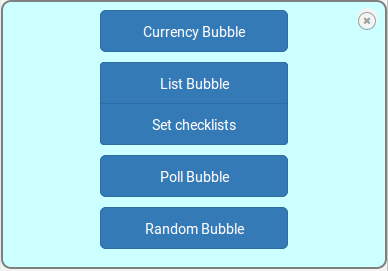
\includegraphics[scale=0.75]{img/menu.png}
\end{center}

Una volta selezionato il pulsante \textbf{Set Checklist} dal menù di creazione delle bolle si aprirà il menù di configurazione della checklist.\\
\begin{center}
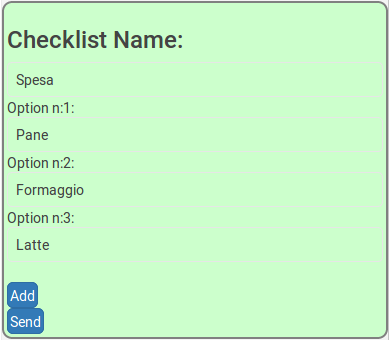
\includegraphics[scale=0.75]{img/checklist_conf.png}
\end{center}

Nel menù di configurazione bisogna inserire il nome della checklist e una o più opzioni.
Per aggiungere una opzione bisogna selezionare il pulsante \textbf{Add}.

Una volta completata la compilazione premendo il pulsante \textbf{Send} la checklist verrà inviata al server e sarà disponibile nella creazione delle liste.
\end{flushleft}

\subsection{Lista}
\begin{flushleft}
La \textit{Lista} è una bolla che permette di creare una lista nella quale è possibile aggiungere degli elementi dalle checklist precedentemente definite.

Per crare una nuova lista selezionare il pulsante \textbf{Lista} dal menù di creazione delle bolle.\\
\begin{center}
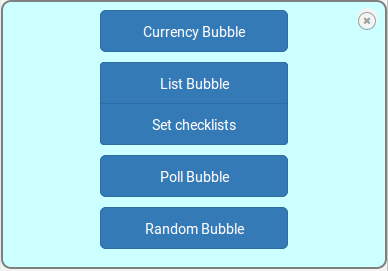
\includegraphics[scale=0.75]{img/menu.png}
\end{center}

Una volta selezionato il pulsante \textbf{Lista} si aprirà il menù di configurazione della lista.\\
\begin{center}
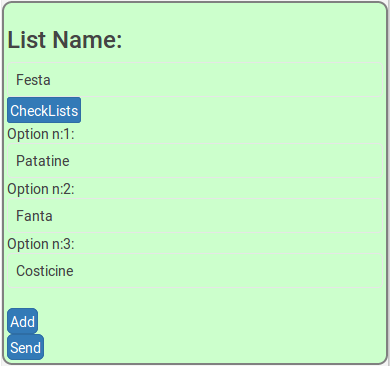
\includegraphics[scale=0.75]{img/list_conf.png}
\end{center}

Nel menù di configurazione bisogna inserire il nome della lista e una o più opzioni.
Per aggiungere una opzione bisogna selezionare il pulsante \textbf{Add} oppure si può selezionare degli elementi da inserire nella lista delle checklist.
Per aprire il menù di selezione delle checklist bisogna premere il pulsante \textbf{Checklists} nel menù di configurazione della lista.\\
\begin{center}
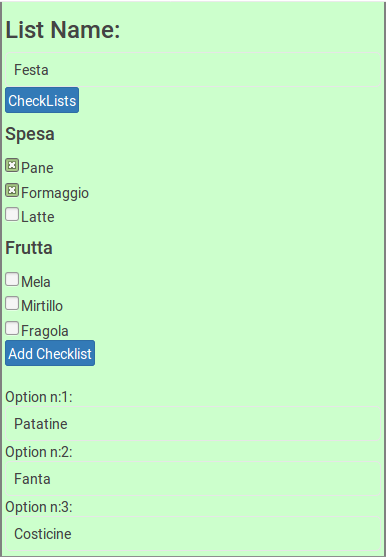
\includegraphics[scale=0.75]{img/list_checklist1.png}
\end{center}

Premendolo nuovamente il menù delle checklist verrà chiuso.
Una volta selezionate le checklist bisogna premere il pulsante \textbf{Add checklist} per aggiungerle alla lista.\\
\begin{center}
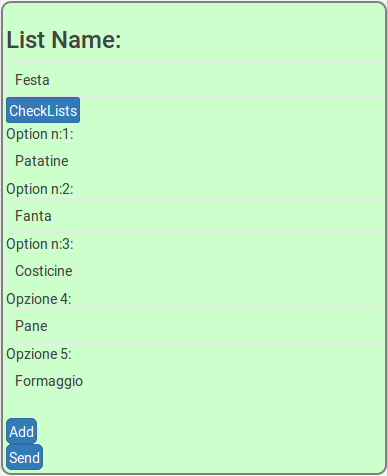
\includegraphics[scale=0.75]{img/list_checklist2.png}
\end{center}

Una volta completata la compilazione premendo il pulsante \textbf{Send} la lista verrà inviata al server e sarà visualizza nell'area contenente le bolle inviate.

\end{flushleft}
